\documentclass[11pt]{article}
\usepackage[margin=2.4cm]{geometry}
\usepackage{booktabs}
\usepackage{amsmath,amssymb}
\usepackage[colorlinks=true,linkcolor=blue]{hyperref}
\usepackage{parskip}
\usepackage{graphicx}
\title{SS-RESfM vs.\ RESfM: Short Summary}
\author{}
\date{September 6, 2026}
\begin{document}
\maketitle
\vspace{-2.5em}

\section*{The summary}

SS-RESfM is RESfM with the supervision removed and nothing else changed --- same
sets-of-sets architecture, tracks, schedule, and robust bundle adjustment, but the
outlier head trains on confident pseudo-labels from the model's own reprojection-error
percentiles instead of COLMAP-derived labels --- and the comparison splits along the
contamination axis. In its curated comfort zone, supervised RESfM keeps at most a modest
edge: in-distribution MegaDepth at $25\%$ contamination, the baseline scores
$0.37\pm0.12$ versus $0.40\pm0.11$ for our test-time-fine-tuned arm (statistically
overlapping, though that arm carries run-to-run noise) or $0.51\pm0.08$ for the
deterministic arms (a ${\sim}38\%$ gap); at $43\%$ with best-case labels the bands
overlap ($5.0\pm2.1$ vs.\ $6.4\pm0.2$); clean Strecha goes to supervision on every
seed ($0.39\pm0.72$ vs.\ ${\sim}2$--$3.2$); and on truly clean \emph{in-distribution} data supervision is a seed lottery
(retrained on the Olsson domain at $0.5\%$, five seeds: $2.03\pm1.86$ --- excellent,
$0.41$--$1.08$, in three seeds, degraded to ${\sim}4$ in two --- while weight+TTT is
stable at $1.60\pm0.81$) --- so SS-RESfM does \emph{not} always win: with sound labels
and curated contamination supervision earns its keep, but even in-domain its advantage
is a three-in-five-seeds advantage.
But it matches supervision at moderate out-of-distribution contamination, beats it
outright where labels cannot be manufactured (plain removal below \emph{every} baseline
seed pair at ${\sim}60\%$: $12.4\pm2.1$ vs.\ $19.2\pm3.4$, and $2\times$ better even
when RESfM is retrained \emph{on} a $60\%$ domain with reference-quality labels ---
proving the failure is caused by labeling, not domain shift), and wins two of the three
clean out-of-distribution splits by $2.5$--$2.9\times$ (BlendedMVS and Olsson, where
every supervised variant lands at $7.4$--$9.1$ versus $2.9$--$3.6$ for every label-free
arm) with a qualitative difference in dependability: the label-free arms land in a
narrow band on every training seed, whereas supervised RESfM collapses on clean OOD in
most seeds under every learning rate, budget, and recipe variant tested. The one-line
version: removing RESfM's labels costs little-to-nothing inside its curated comfort zone
(and Strecha), and buys robustness --- and above all \emph{reliability} --- everywhere
labels are unsound or unavailable, which is exactly where robust SfM is needed.

\section*{What ``RESfM collapses'' means}

``Collapse'' is not divergence or a crash --- the network trains normally and
reconstructs its training distribution well. It is a \emph{silent generalization
failure on the easiest possible test}: Olsson, $39$ essentially outlier-free scenes
($0.5\%$ measured contamination), where a method that merely ignored its outlier head
should do fine. Every MegaDepth-trained \emph{supervised} variant we test --- the
authors' released checkpoint ($9.10$), the authors-faithful retrain ($8.77$), and our
controlled from-scratch retrains ($7.4\pm2.6$) --- lands at a translation error of
$7.4$--$9.1$, versus $2.9$--$3.6$ for every label-free arm and $3.15$ for classical
GLOMAP. It is seed-dependent but dominant ($4$ of $5$ training seeds collapse; one
escapes to $2.32$), and it survives every learning rate, epoch budget, and recipe
variant we try. Crucially it is \emph{not} a domain-shift story: RESfM retrained
in-distribution on the Olsson domain improves to $2.03\pm1.86$ over five seeds
(bimodal: $0.41$--$1.08$ in three, ${\sim}4$ in two) --- in-domain labels remove the
bulk of the collapse, so the supervised outlier
head, fit to MegaDepth's label distribution, actively misclassifies on clean
out-of-distribution scenes, while the self-supervised head adapts because its
pseudo-labels are recomputed from the test-time reprojection-error distribution itself.

\section*{The picture in one figure}

\begin{center}
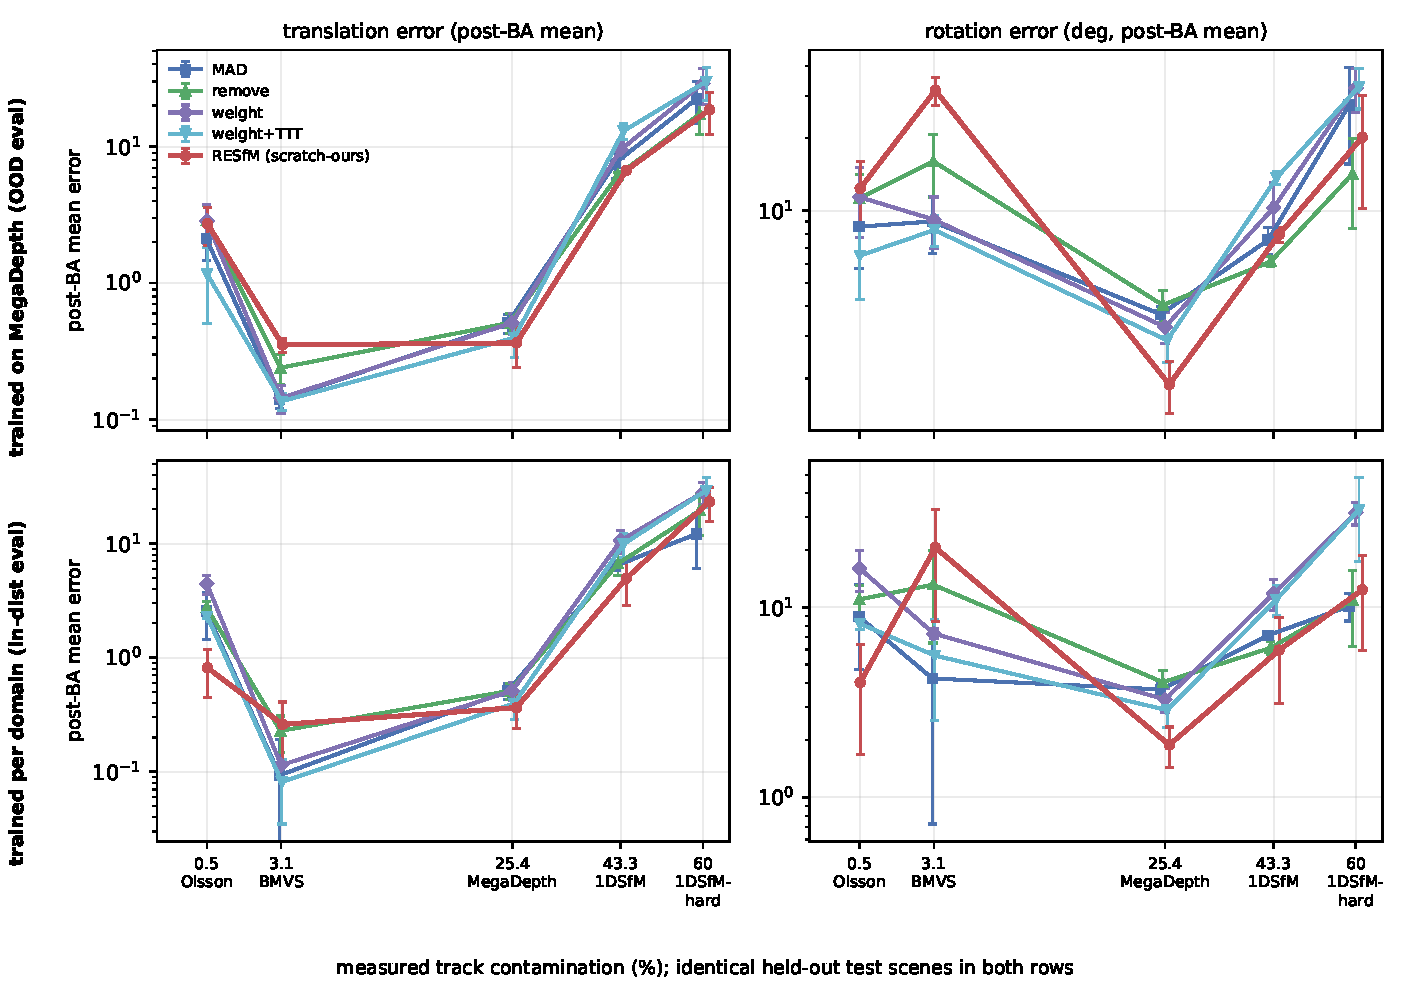
\includegraphics[width=\linewidth]{fig_4panel_scratch.pdf}
\end{center}
\noindent\emph{Columns:} translation / rotation (post-BA means, log scale).
\emph{Top row:} all methods trained on MegaDepth, evaluated out-of-distribution on
each domain's held-out test scenes. \emph{Bottom row:} trained on each domain itself
(supervised with best-case GT-derived labels), evaluated in-distribution on the same
scenes. The red supervised line is RESfM-from-scratch (our controlled anchor) in the
top row and the in-domain retrain in the bottom row (MegaDepth anchor point shared);
label-free arms carry five-seed bands. In-domain retraining helps supervision at
$0.5\%$ (from full collapse to a seed lottery: excellent in three of five seeds,
degraded in two) and at $43\%$, does nothing at $3.1\%$ (the dead zone ---
rotation-first in both rows), and worsens at $60\%$, while the label-free arms barely
move between rows: they have no labels to gain from. The top row also shows Strecha ($1.7\%$, full four-scene OOD eval; no bottom-row counterpart --- its same-protocol in-distribution split leaves a single uninformative test scene): supervision's clean-OOD win there is visible in both columns. Analogous figures exist with the
authors-faithful retrain and the released checkpoint as the supervised line; the
verdicts are unchanged. (Test-scene restriction caveats: the $8$ Olsson held-out
scenes exclude most of the clean-OOD collapse scenes, and the $43\%$ point is a
three-scene mean including the Ellis Island failure scene.)

\section*{Why five seeds (seed-additivity fails)}

If the training seed shifted all models equally, relative differences would be
seed-invariant and one seed would suffice --- the implicit assumption of prior work in
this benchmark family, which fixes a single seed. Tested directly on the saved
per-scene results ($98$ scene-cells, five seeds), the assumption fails: the sign of the
supervised-vs-MAD difference flips across seeds in $67\%$ of scenes, the across-seed
spread of the difference matches or exceeds the margin itself, and the
\emph{dataset-level} verdict flips across seeds on four of six datasets (MegaDepth,
1DSfM, 1DSfM-hard, and Olsson --- where the one escape seed briefly hands supervision
the win); only Strecha and BlendedMVS are seed-invariant, and those are exactly the two
cells stated as every-seed claims. A single-seed study can therefore reverse the
headline conclusion on most datasets --- which is why every comparison in this project
carries five-training-seed bands, and the strongest claims are verified over all seed
pairings. (Evaluation seeds, by contrast, are a shared negligible offset, $\pm0.008$
--- replicating over them is unnecessary, and we don't.)

\section*{The four RESfM reference points}

All four supervised reference points appear in the paper's main table; translation
error (mean), lower is better. The controlled comparison arm is RESfM-scratch:
identical tracks, schedule, and BA to our label-free arms, with checkpoint selection by
our label-free reprojection-error criterion (which \emph{favors} the baseline relative
to the authors' own Accuracy-based selection --- MegaDepth $0.37$ vs.\ $0.50$).

\begin{center}
\small
\begin{tabular}{lcccccc}
\toprule
RESfM variant & MegaDepth & 1DSfM & 1DSfM-hard & Strecha & BMVS & Olsson\\
 & (25\%) & (43\%) & (60\%) & (1.7\%) & (3.1\%) & (0.5\%)\\
\midrule
Paper (reported)              & 0.169 & -- & -- & -- & -- & --\\
Released (authors' weights)   & 0.203$\pm$0.008 & 10.71 & 15.29 & 0.20 & 0.33 & 9.10\\
From scratch, faithful (authors' ckpt sel.) & 0.496 & 9.75 & 17.58 & 0.14 & 0.37 & 8.77\\
From scratch, our reproj-error ckpt sel.    & 0.37$\pm$0.12 & 10.5$\pm$1.5 & 19.2$\pm$3.4 & 0.39$\pm$0.72 & 0.35$\pm$0.04 & 7.4$\pm$2.6\\
\midrule
SS-RESfM best label-free arm  & 0.40$\pm$0.11 & 8.9$\pm$1.2 & 12.4$\pm$2.1 & 1.97$\pm$0.09 & 0.14$\pm$0.02 & 2.9$\pm$0.3\\
\bottomrule
\end{tabular}
\end{center}

Reading the four rows: the \emph{paper} number ($0.169$) is not reproducible even from
the authors' own released weights in our harness ($0.209$, confirmed under their pinned
software stack); the \emph{released} checkpoint is the strongest in-distribution but
collapses on Olsson like every other supervised variant ($9.10$) --- so the collapse is
not an artifact of our retraining; the \emph{faithful} from-scratch retrain (authors'
own checkpoint-selection metric) is the weakest in distribution ($0.496$), showing our
selection deviation helps the baseline, not us; and \emph{from-scratch with our
selection} is the controlled anchor used for all seed-band claims. Against whichever
row one prefers, the label-free story is unchanged: supervision holds MegaDepth and
Strecha; label-free wins the high-contamination regime, BlendedMVS, and Olsson, and is
the only recipe that never collapses.

\end{document}
